\documentclass[11pt,a4paper,ngerman]{article}
\usepackage[bottom=2.5cm,top=2.5cm]{geometry} 
\usepackage{babel}
\usepackage[utf8]{inputenc} 
\usepackage[T1]{fontenc} 
\usepackage{ae} 
\usepackage{amssymb} 
\usepackage{amsmath} 
\usepackage{graphicx}
\usepackage{fancyhdr}
\usepackage{fancyref}
\usepackage{listings}
\usepackage{xcolor}
\usepackage{paralist}

\usepackage[pdftex, bookmarks=false, pdfstartview={FitH}, linkbordercolor=white]{hyperref}
\usepackage{fancyhdr}
\pagestyle{fancy}
\fancyhead[C]{Approximation Algorithms}
\fancyhead[L]{Exercise sheet 1}
\fancyhead[R]{SoSe 2012}
\fancyfoot{}
\fancyfoot[L]{}
\fancyfoot[C]{\thepage \hspace{1px} of \pageref{LastPage}}
\renewcommand{\footrulewidth}{0.5pt}
\renewcommand{\headrulewidth}{0.5pt}
\setlength{\parindent}{0pt} 
\setlength{\headheight}{0pt}

\date{}
\title{Max Wisniewski , Paul Podlech}
\author{Dozent : Panos Giannopoulos}

\newcommand{\claim}{\addtocounter{claims}{1} \bfseries Claim \arabic{claims}}
\newcommand{\proof}{\bfseries Proof}


\begin{document}

\lstset{language=Pascal, basicstyle=\ttfamily\fontsize{10pt}{10pt}\selectfont\upshape, commentstyle=\rmfamily\slshape, keywordstyle=\rmfamily\bfseries, breaklines=true, frame=single, xleftmargin=3mm, xrightmargin=3mm, tabsize=2}

\renewcommand{\figurename}{Figure}
\newcounter{claims}

\maketitle
\thispagestyle{fancy}

%% ------------------------------------------------------
%%                     Exercise 1
%% ------------------------------------------------------

\section*{Exercise 1}

Consider the 2-approximation algorithm for the cardinality (i.e. unweighted) Vertex Cover problem that is based on computing a Maximal Matching. What approximation factor does it give for the general weighted vertex cover problem, where the vertices have arbitrary positive weights?\\
\textbf{Solution:}\\
Let $G(V,E)$ be the graph, $C$ the approximated vertexcover, OPT the Minimum Vertex Cover, $\min$ be the vertex with the minimal value and $\max$ the maximal value.

\begin{description}

    \item{\claim} $ |C| \leq 2 \cdot \frac{\max}{\min} \cdot |OPT| $.
    \item{\proof} 

For every node, that is in $C$ the relative error we made is obviously at most $\frac{\max}{\min}$. From the cardinality problem we know, that this algorithm will take at most $2$ times the vertices. Now holds
$$
\begin{array}{rcl}
OPT &=& \underset{v\in OPT}{\sum} w(v)\\
    &\leq& \underset{v \in OPT}{\sum} \frac{\max}{\min}\\
    &=& \frac{\max}{\min} \underset{v \in OPT}{\sum} 1\\
    &\leq& 2\frac{\max}{\min}\cdot |C|
\end{array}
$$
\end{description}

%%--------------------------------------------------
%%		Exercise 2
%% -------------------------------------------------

\section*{Exercise 2}
Consider the following greedy algorithm for carinality Vertex Cover:
\begin{itemize}
    \setlength{\itemsep}{0pt}
    \setlength{\parsep}{0pt}
	\item Input : Graph $G(V,E)$
	\item $C := \emptyset$
	\item While $C$ is not a vertex cover of $G$
		\begin{itemize}
			\item let $u$ be the vertex incident to the most uncovered edges
			\item $C := C \cup \{ u \}$
		\end{itemize}
	\item return $C$
\end{itemize}
\begin{figure}[!b]
	\centering
	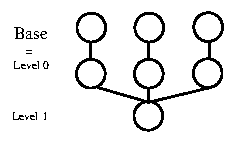
\includegraphics[width=1.75in]{ex2_anchor}
	\caption{Anchor of the graph familiy ($G_1$)}
	\label{fig:ex2:anchor}
\end{figure}

Is this a constant-factor approximation algorithm?\\
\textbf{Solution}
\begin{description}
	\item{\claim} The algorithm is not a constant-factor approximation algorithm.
	\item{\proof}


We construct a family of graphs that have a factor, dependend in the amount of vertices.\\
Let $G_n(V_n,E_n)$ be a family of graphs constructed as inductiv as followed:\\
$G_1(V_1,E_1)$ is a graph of the pairwise connected vertices and one vertex, that has a edge to one vertex of each pair. In figure \ref{fig:ex2:anchor} the graph is visualized.\\
Now for the Induction $G_i$ we take three graph of $G_{i-1}$. Further we add a number of new vertices to the graph and connect each of these vertices with each vertex in every baselayer in the three $G_{i-1}$ graphs, therefore the degree of these vertices will be $3^i$. The constructed graph looks like the example in figure \ref{fig:ex2:example} for the $G_2$.\\
The number of new vertices we will add must be as large as possible, but only that much, that our $3^i$ vertices in the baselevel will have at most the degree $3^i - 1$. From this we construct two formulas $\eta$ for the amount of vertices on level $k$ and $\Psi$ for all nodes (the pairs in the baselevel count as 1 per pair).


\begin{figure}[!b]
	\centering
	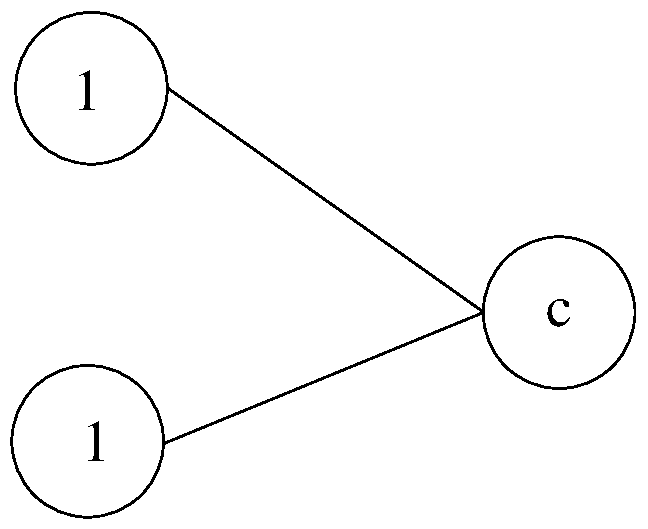
\includegraphics[width=\textwidth]{ex2_counter}
	\caption{Example for the graph $G_2$ of the family in exercise 2}
	\label{fig:ex2:example}
\end{figure}

$$
\begin{array}{rcl}
\eta & \; : \; & \mathbb{N}  \longrightarrow  \mathbb{N}\\
0 & \mapsto & 1\\
i & \mapsto & 3^i - \left( \underset{k=0}{\overset{i-1}{\sum}} \eta (k) \right) - 1 \quad , i>0 
\vspace{12pt}\\
\Psi & \; : \;&  \mathbb{N} \longrightarrow \mathbb{N}\\
i & \mapsto & 3^i + \underset{k=1}{\overset{i-1}{\sum}} 3^{k-1} \times \eta (i - k - 1)
\end{array}
$$

As one can easily see, the Vertex Cover must contain one vertex of each pair in the base level at least. Because every other edge is connected to the baselevel, the Minimum Vertex Cover will contain exactly one vertex (the one every edge is connected to) from each pair. So the OPT is $3^n$ for $G_n$.\\

The algorithm instead will take $\Psi (n)$ for $G_n$. This is, because we constructed the graph the way, that the vertices with the most uncovered edges are the one in the highest level. The base level will have at most one degree less, then the ones in the top level. After alle the toplevel vertices are taken for the Vertex Cover, the resulting graph will be three times $G_{n-1}$, because we could erase all taken nodes and edges connected to them, because the algorithm will no longer concern them as they all are covered.\\
The vertices we need for the vertex cover therefore will only be taken, after we took alle extra vertices from every level.\\

To proof this is not a constant-factor approximation we have to show, that $\frac{\Psi (n)}{ 3^n }$ is unbounded.
$$
\begin{array}{rcl}
\frac{\Psi(n)}{3^n} &=& 3^n + \underset{k=1}{\overset{n-1}{\sum}} 3^{k-1} \times \eta (n - k - 1) \cdot \frac{1}{3^n}\\
&=& 1 + \underset{k=1}{\overset{n-1}{\sum}} 3^{k - 1 - n} \times \eta (n - k - 1)
\end{array}
$$

For the result we must only concern ourselves with the sum. As we now through simple analysis these row diverge if the inner sequence does not converge against zero. Because we only sum up positive values the row would diverge against positive infinity.\\

\begin{description}
	\item{\claim} $\forall n > 0 : \eta (n) = 3^n - 3^{n-1}$
	\item{\proof} Induction over $n$\\
	\begin{description}
		\item{\bfseries I.A.} $n=1$\\
			$\eta (1) = 3^1 - 1 = 3^1 - 3^0$
		\item{\bfseries I.S.} $n \rightarrow n+1$\\
			$$
				\begin{array}{rcl}
					\eta(n+1) &=& 3^{n+1} - \left( \underset{k=0}{\overset{n}{\sum}} \eta (k) \right) - 1\\
						&\overset{\text{I.P.}}{=}& 3^{n+1} -  \left( \underset{k=0}{\overset{n}{\sum}} 3^k - 3^{k-1} \right) - 1\\
						&=& 3^{n+1} - 3^n - \left( \underset{k=1}{\overset{n-1}{\sum}} 3^k - 3^k \right)\\
						&=& 3^{n+1} - 3^n
				\end{array}
			$$
\mbox{}\hfill $\square$
	\end{description}
\end{description}

If we take this claim into consideration
$$
\begin{array}{rcl}
\frac{\Psi(n)}{3^n} &=& 1 + \underset{k=1}{\overset{n-1}{\sum}} 3^{k - 1 - n} \cdot ( (3^{n-k-1} - 3^{n-k-2})\\
	&=& 1 + \underset{k=1}{\overset{n-1}{\sum}} 3^{k-1-n + n - k -1} - 3^{k - 1 - n + n - k -2}\\
	&=& 1 + \underset{k=1}{\overset{n-1}{\sum}} 3^{-2} - 3^{-3}\\
	&=& 1 + \underset{k=1}{\overset{n-1}{\sum}} \frac{2}{27}
\end{array}
$$
holds.

The inner sequence is a constant sequence and is never zero. Therefore the row does in fact diverge against positive infinity.\\

We proofed, that the approximation is not constant. The $\delta$ will be in $\Omega (\log n)$ because we have an lineare error growth over an exponential growth of vertices. \mbox{} \hfill $\square$

\end{description}



%% -------------------------------------------------------
%%			Exercise 3
%% ------------------------------------------------------

\section*{Exercise 3}
Consider the following approximation algorithm for the cardinality Vertex Cover problem: Find a depth first search tree $T$ in the given input graph $G$, and return the set $C$ of all the nonleaf vertices of $T$. Show that this is also a 2-approximation algorithm.\\
\textbf{Solution}\\
Let $\mathfrak{D}$ be the Algorithm described above. I assume the Graph $G$ is connected. Otherwise we can find a simple counterexample.

\begin{description}
	\item{\claim} The set $C$ returned by $\mathfrak{D}$ is a vertex cover.
	\item{\proof}

Let $G(V,E)$ be a valid instance for this problem and $T$ the DFS tree generated by $\mathfrak{D}$. A DFS tree in a Connected Graph visits all nodes. If not, there would exist an edge from a visited node to an unvisited one alongside the algorithm should have taken its path.\\

Let e = (i,j) be an uncovered edge. This edge can only be an edge between two leafs, because every other vertex is in the cover. But \emph{dfs} will inspect, after it visits a vertex first every child recursivly. Therefore either $i$ or $j$ would have to be an inner vertex.

\mbox{} \hfill $\square$  


	\item{\claim} Let $G(V,E)$ be a graph and $T(V,E')$ be a spanning tree of $G$. \\If $I = \{v \in V \; | \; \deg_T (v) \geq 2\}$ is a Vertex Cover, then 
			$|I| \leq 2 \times OPT$ holds.
	\item{\proof}

Let $n =|V|$ the amount of vertices, $i = |I|$ the amount of inner vertices.\\
Because every vertex except for the root in the tree has exactly one parent. So the amount of tree edges is $n-1$ and the amount of edges in between the nonleaf vertices is $i-1$.\\
Because of that fact the Vertex Cover has to be at least $\frac{i-1}{2}$ times large as the amount of inner vertices $i$. So the optimal solution $OPT \geq \frac{i-1}{2}$.
Considering that
$$i \leq 2 \cdot \frac{i - 1}{2} + \frac{1}{2} \leq 2 \cdot OPT + \frac{1}{2}$$ holds, 
but both the optimal and the feasible solution of $\mathfrak{D}$ are natural Numbers, so the equation
$$
i \leq 2 \cdot OPT
$$
holds.\mbox{} \hfill $\square$

	\item{\claim} $\mathfrak{D}$ is a 2-approximation-algorithm.
	\item{\proof} Directly follows from \emph{claim 5} and \emph{calim 6}.

\mbox{}\hfill $\square$
\end{description}

\label{LastPage}

\end{document}
